\chapter{血糖预测中动力系统模型的发展}
\section{糖尿病简介}
糖尿病是一种由于胰岛素分泌不足或者人体内不能充分利用胰岛素,以高血糖,尿液中含有葡萄糖等为标志的慢性疾病。糖尿病的症状主要表现为“三多一少”,即多饮、多尿、多食和体重下降。原因是因为体内血糖过高,需要经常将尿液排出,因此会引起体内缺水,需要多喝水,由于体内血糖过高,人体对血糖的利用程度也会下降,因此可能还有无意识体重减轻和多食的症状。

目前糖尿病主要有三种类型以及一种预发病类型\cite{whoDiabetes}:
\begin{enumerate}
    \item 一型糖尿病(Type 1 Diabetes, T1D):一型糖尿病是由于胰岛素分泌不足,导致血糖过高。一型糖尿病通常发生在年轻人身上,可能是由于自身免疫系统攻击胰岛素生成细胞,导致胰岛素生成细胞减少,从而导致胰岛素分泌不足。目前尚不清楚病因,但可能与遗传、环境等因素有关。多见于高收入地区,一般于青少年时期就开始发病。
    \item 二型糖尿病(Type 2 Diabetes, T2D):二型糖尿病是由于人体细胞对胰岛素的敏感性降低,导致胰岛素不能充分发挥作用,从而导致血糖过高。有的是因为胰岛素受体受损,发病原因可能与遗传、运动不足以及超重有关。二型糖尿病是最常见的糖尿病类型,并且患者日益增多。
    \item 妊娠糖尿病(Gestational Diabetes Mellitus)
    :妊娠糖尿病是指妊娠期间发生的糖尿病。此时血糖值高于正常范围但低于糖尿病患者的水平。妊娠糖尿病可能会增加母亲和胎儿的健康风险,但通过控制饮食和运动可以有效控制。
    \item 糖耐量受损(Impaired Glucose Tolerance, IGT)和空腹血糖受损(Impaired Fasting Glucose, IFG):IGT和IFG是正常状态与糖尿病之间过渡的中间状态。患有IGT或IFG的人群高度可能会发展为2型糖尿病。
\end{enumerate}

对于这种病症,在有前兆时提前预防是最佳的治疗方法,因此我们需要建立一个动力系统模型来预测人体内的血糖数值,以此来衡量这个人是否有风险患病等。

\section{葡萄糖动力系统}
在后吸收状态下,葡萄糖由肝脏和肾脏释放到血液中,被体内所有细胞从间质液中移除,并分布到许多生理组分中(例如,动脉血、静脉血、脑脊液、间质液)。我们可以通过以下微分方程来描述葡萄糖动力系统\cite{bergman1979quantitative}:

\begin{equation}\label{1}
    \frac{dG}{dt} = \text{Production} - \text{Uptake},
\end{equation}
其中$G$是血液中的葡萄糖浓度,$t$是时间,Production是葡萄糖生成速率,Uptake是葡萄糖摄取速率(也可以理解为血液中葡萄糖的消耗速率)。

葡萄糖产生和摄取的速率主要取决于血糖和胰岛素水平。这些关系已经通过葡萄糖夹持技术进行了实验定义,该技术允许在各种稳态血糖和胰岛素水平下测量葡萄糖产生和摄取速率\cite{bergman1985assessment}。在恒定胰岛素水平下,葡萄糖产生减少而摄取增加,两者都与血糖水平线性相关\cite{best1981glucose}。这些线性依赖的斜率是“葡萄糖效力”的参数。因此,我们可以将葡萄糖产生和摄取速率表示为:

\begin{equation}\label{2}
    \text{Production} = P_0 -(E_{G0P} + S_{IP} \times I) \times G,
\end{equation}
\begin{equation}\label{3}
    \text{Uptake} = U_0 + (E_{G0U} + S_{IU} \times I) \times G,
\end{equation}

其中$P_0$和$U_0$是零葡萄糖时的葡萄糖产生和摄取速率,\(E_{G0P}\)和\(E_{G0U}\)分别是产生和摄取的零胰岛素葡萄糖效力,\(S_{IP}\)和\(S_{IU}\)分别是产生和摄取的胰岛素敏感性,$I$代表血胰岛素浓度。将方程(\ref{2})和(\ref{3})代入方程(\ref{1}),我们得到

\begin{equation}
    \frac{dG}{dt} = R_0 -(E_{G0} + S_I \times I) \times G,
\end{equation}
其中$R_0$($=P_0-U_0$)是零葡萄糖时葡萄糖的净产生速率,\(E_{G0}\)($=E_{G0p}+E_{G0U}$)是零胰岛素时的总葡萄糖效力,\(S_I\)($=S_{IP}-S_{IU}$)是总胰岛素敏感性\cite{topp2000model}。

再考虑体内的肝糖原水解产生的葡萄糖,最终可以得到
\begin{equation}
    \frac{dG}{dt} = R_0 -(E_{G0} + S_I \times I) \times G+\frac{K_0}{K_1+I^p},
\end{equation}
其中$K_0,K_1,p$为与肝糖原分解产生葡萄糖相关的常数\cite{bridgewater2020amplitude}。
\section{胰岛素动力系统}
胰岛素是一种由胰$\beta$细胞分泌的激素,是调节血糖水平的关键因素之一。它在体内的主要作用是促进组织对葡萄糖的摄取和利用,从而降低血糖水平。当血糖水平升高时,胰$\beta$细胞会释放胰岛素进入血液循环,分布到几个组分中(例如,门静脉、外周血和间质液),刺激肝脏、肌肉和脂肪组织中的细胞摄取和存储葡萄糖,从而使血糖水平下降。

胰岛素在人体内最后会被肝脏、肾脏和胰岛素受体清除。我们可以通过以下微分方程来描述胰岛素动力系统:

\begin{equation}\label{4}
    \frac{dI}{dt} = \text{Secretion} - \text{Clearance},
\end{equation}
其中Secretion表示胰岛素分泌速率,Clearance表示胰岛素清楚速率。

我们假设胰岛素清除速率为\(kI\),其中$k$是代表肝脏、肾脏和胰岛素受体中胰岛素摄取的清除常数。

当系统处于近稳态时,胰岛素清除速率与血液胰岛素水平成正比。我们假设胰岛素分泌速率模拟为葡萄糖水平的S形函数\cite{topp2000model}。因此,我们假设

\begin{equation}\label{5}
    \text{Secretion} = \frac{\beta\sigma G^2}{(\alpha + G^2)},
\end{equation}

其中$\beta$是胰$\beta$细胞的质量。所有$\beta$细胞被假定以相同的最大速率$\sigma$分泌胰岛素,\(G^2/(\alpha + G^2)\)是一个带有系数$2$的Hill函数,描述了从$0$到$1$的S形范围,在$G=\alpha^{\frac{1}{2}}$时达到其最大值的一半。将方程(\ref{5})代入方程(\ref{4}),我们得到控制胰岛素动力学的方程:

\begin{equation}
    \frac{dI}{dt} = \frac{\beta\sigma G^2}{(\alpha + G^2)} - kI.
\end{equation}

\section{胰\(\beta\)细胞动力系统}
胰$\beta$细胞是胰岛中的一种细胞类型,位于胰岛的中心部位,通常被称为“Langerhans岛”。这些细胞是胰岛素的主要生产者,其功能是根据体内的血糖水平分泌胰岛素。当血糖水平升高时,胰$\beta$细胞受到刺激,释放更多的胰岛素以帮助降低血糖水平。胰$\beta$细胞的功能障碍或数量减少可能会导致胰岛素分泌不足,从而引发糖尿病等代谢性疾病。

不同的胰$\beta$细胞含量会影响血糖平衡点的位置,在其余参数相同的情况下,如图\ref{fig:nullcline}所示,当胰$\beta$细胞数量增加时,不动点位置会向右下方移动,即最后平衡时刻血糖含量较低,胰岛素含量较高。


\begin{figure}[H]
    \centering
    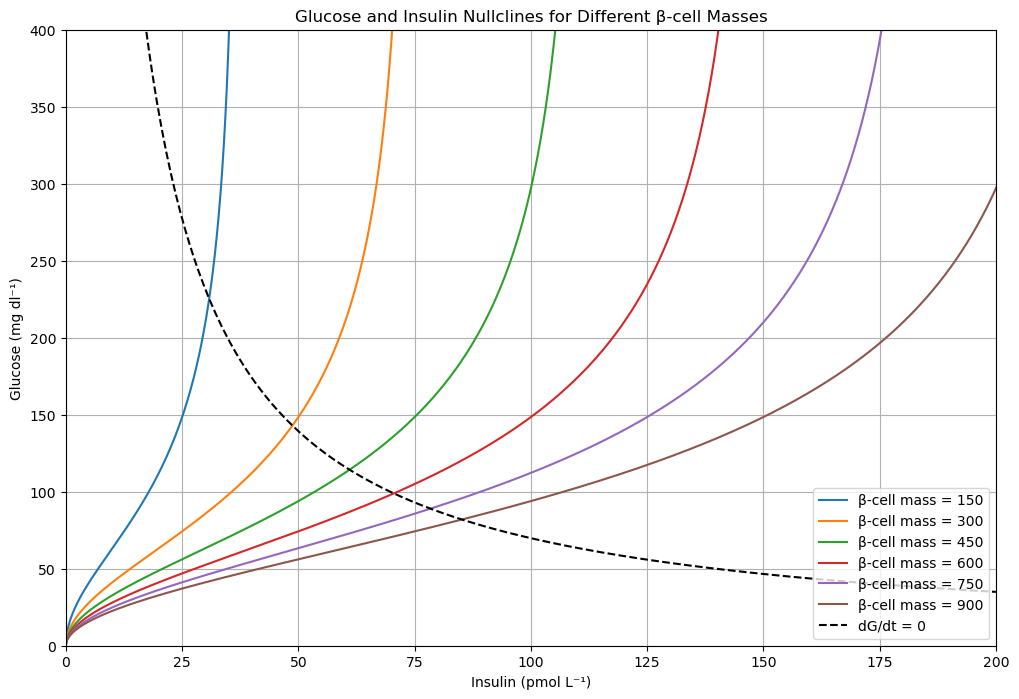
\includegraphics[width=0.7\textwidth]{Img/nullcline.png}
    \centering\bicaption{不同胰β细胞下动力系统模型不动点位置的变化。}{The change of the equilibrium point position of the dynamic system model under different pancreatic β cell.}
    \label{fig:nullcline}
\end{figure}

对于一些特定的胰$\beta$细胞的值,整个葡萄糖-胰岛素-胰$\beta$细胞动力系统的相图如下图所示:
\begin{figure}[H]
    \begin{minipage}[t]{0.5\textwidth}
        \centering
        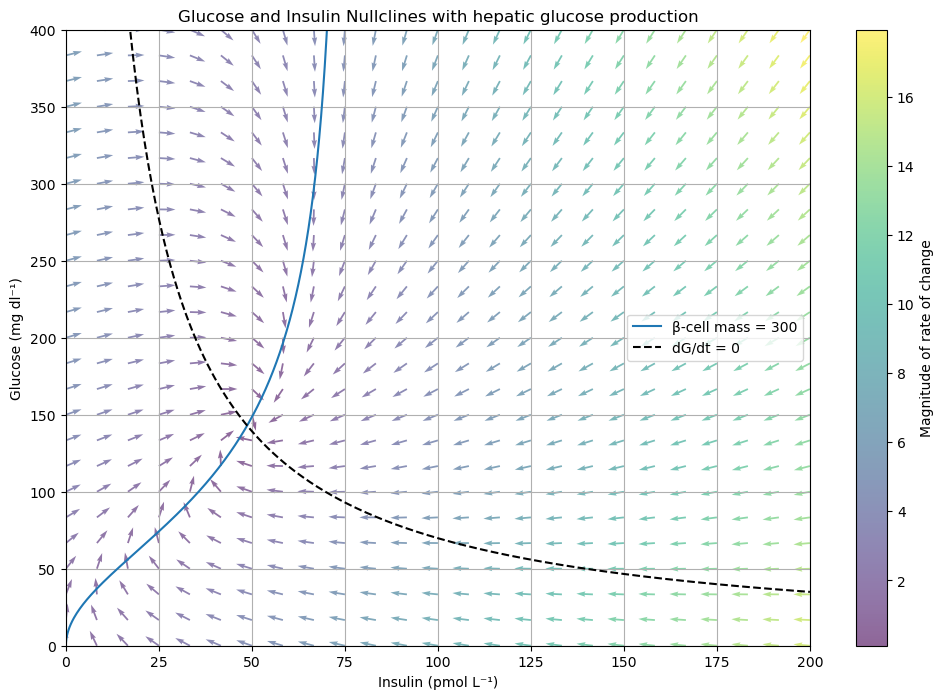
\includegraphics[width=0.9\textwidth]{Img/phase_300.png}
    \end{minipage}
    \begin{minipage}[t]{0.5\textwidth}
        \centering
        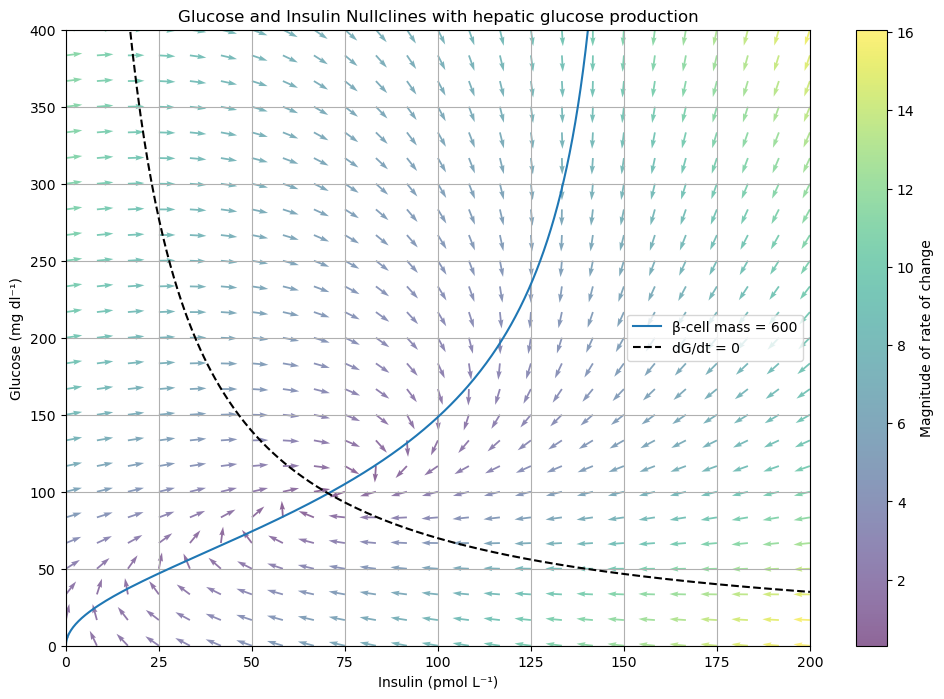
\includegraphics[width=0.9\textwidth]{Img/phase_600.png}
    \end{minipage}
    \bicaption{不同胰\(\beta\)细胞下动力系统模型相图。}{The phase diagram of the dynamic system model under different pancreatic \(\beta\) cell.}
    \label{fig:phase}
\end{figure}

尽管胰$\beta$细胞在胰腺中分布复杂,但$\beta$细胞质量动态可以用单一组分模型定量化,新的$\beta$细胞可以通过现有$\beta$细胞的复制、新生(干细胞的复制和分化)和其他细胞的转分化来形成。目前,无法量化新生和转分化的速率。然而,除了在发育期间和在极端生理或化学诱导创伤反应中,这些可以忽略不计\cite{finegood1995dynamics}。基于这些原因,新生和转分化未纳入当前模型,且生成的$\beta$细胞被假定等于所有复制的$\beta$细胞。

我们可以通过以下微分方程来描述胰$\beta$细胞动力系统:
\begin{equation}
    \frac{d\beta}{dt} = (-d_0+r_1G-r_2G^2)\beta,
\end{equation}

其中$d_0$是零血糖时$\beta$细胞的自然死亡率,$r_1$和$r_2$是两个常系数\cite{topp2000model}。

在此动力系统模型下,我们可以得到胰$\beta$细胞数量与血糖浓度的变化规律。
\begin{figure}[H]
    \centering
    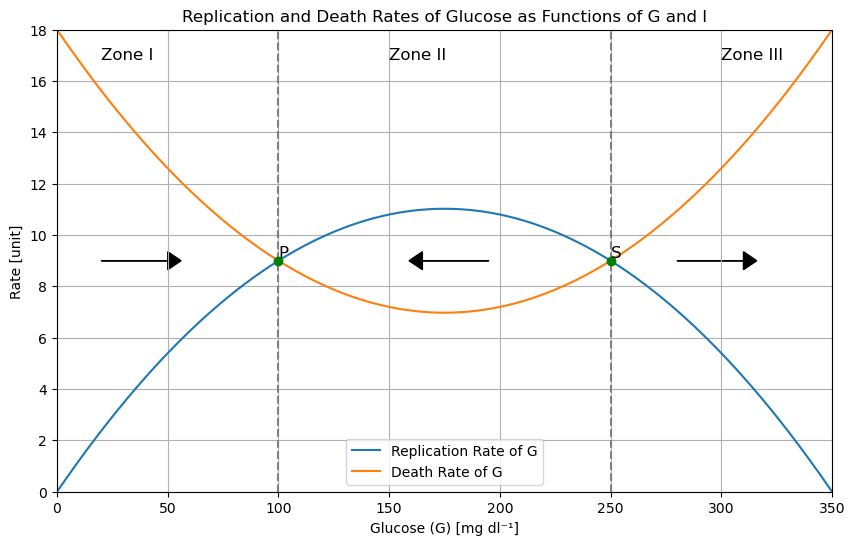
\includegraphics[width=0.7\textwidth]{Img/betarate.png}
    \bicaption{胰$\beta$细胞生成率和死亡率与血糖浓度的变化规律。}{The change of pancreatic \(\beta\) cell generation rate and death rate with blood glucose concentration.}
    \label{fig:beta}
\end{figure}

这时整个血糖-胰岛素-胰$\beta$细胞动力系统模型的相图如图\ref{fig:3dphase}所示。
\begin{figure}[H]
    \centering
    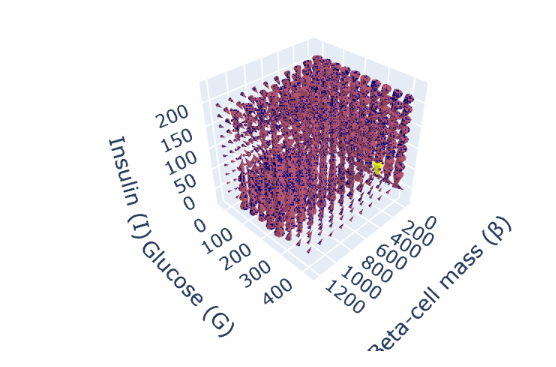
\includegraphics[width=0.7\textwidth]{Img/3dphase.png}
    \bicaption{血糖-胰岛素-胰$\beta$细胞动力系统模型相图。}{The phase diagram of the glucose-insulin-pancreatic \(\beta\) cell dynamic system model.}
    \label{fig:3dphase}
\end{figure}

考察胰$\beta$细胞-胰岛素-血糖浓度构成的动力系统
\begin{equation}
    \begin{aligned}
        \dot{G}     & = a_0-a_1G-a_2GI+\frac{a_3}{a_4+I^p} ,      \\
        \dot{I}     & = \frac{b_1\beta G^2}{G^2 + b_2^2} - b_3 I ,\\
        \dot{\beta} & = (-d_0+r_1G-r_2G^2)\beta,
    \end{aligned}
\end{equation}
我们可以得到如下不动点方程组
\begin{equation}\label{fixequation}
    \begin{aligned}
        a_0-a_1G^*-a_2G^*I^*+\frac{a_3}{a_4+{I^*}^p}     & =0, \\
        \frac{b_1\beta {G^*}^2}{G^{*2} + b_2^2} - b_3I^* & =0, \\
        (-d_0+r_1G^*-r_2{G^*}^2)\beta^*                  & =0,
    \end{aligned}
\end{equation}
对于
\begin{equation}\label{G^*}
    -d_0+r_1G^*-r_2{G^*}^2=0,
\end{equation}
显然胰$\beta$细胞不会单调递增或递减,因此方程\ref{G^*}一定有两个正实数解,解出的$G^*$,将其带入方程组\ref{fixequation}的第一行我们可以得到对应的$I^*$,再通过第二行可解得对应的$\beta^*$,因此该动力系统模型存在至少两个不动点。对于不动点$(G^*,I^*,\beta^*)$,线性化该动力系统模型可得
\begin{equation}\label{linear}
    \begin{pmatrix}
        \dot{G} \\
        \dot{I} \\
        \dot{\beta}
    \end{pmatrix}=\begin{pmatrix}
        -a_1-a_2I^*                            & -a_2G^*-\frac{pa_3(I^*)^{p-1}}{(a_4+(I^*)^p)^2} & 0                                  \\
        \frac{2b_1\beta^*G^*}{(G^*)^2 + b_2^2} & -b_3                                            & \frac{b_1(G^*)^2}{(G^*)^2 + b_2^2} \\
        r_1\beta^*-2r_2G^*\beta^*              & 0                                               & 0
    \end{pmatrix}\begin{pmatrix}
        G-G^* \\
        I-I^* \\
        \beta-\beta^*
    \end{pmatrix},
\end{equation}

对于方程\ref{G^*}中较小的解$G_1^*$,线性化系统\ref{linear}中的雅可比矩阵的行列式为
\begin{equation}
    \begin{aligned}
        \det&\begin{pmatrix}
            -a_1-a_2I^*                                & -a_2G_1^*-\frac{pa_3(I^*)^{p-1}}{(a_4+(I^*)^p)^2} & 0                                      \\
            \frac{2b_1\beta^*G_1^*}{(G_1^*)^2 + b_2^2} & -b_3                                              & \frac{b_1(G_1^*)^2}{(G_1^*)^2 + b_2^2} \\
            r_1\beta^*-2r_2G_1^*\beta^*                & 0                                                 & 0
        \end{pmatrix}\\
        &=(r_1\beta^*-2r_2G_1^*\beta^*)(-a_2G_1^*-\frac{pa_3(I^*)^{p-1}}{(a_4+(I^*)^p)^2})( \frac{b_1(G_1^*)^2}{(G_1^*)^2 + b_2^2}),
    \end{aligned}
\end{equation}
我们有
\begin{equation}
    \begin{aligned}
        r_1\beta^*-2r_2G_1^*\beta^*                       & >0, \\
        -a_2G_1^*-\frac{pa_3(I^*)^{p-1}}{(a_4+(I^*)^p)^2} & <0, \\
        \frac{b_1(G_1^*)^2}{(G_1^*)^2 + b_2^2}            & >0,
    \end{aligned}
\end{equation}
因此\begin{equation}
    \det\begin{pmatrix}
        -a_1-a_2I^*                                & -a_2G_1^*-\frac{pa_3(I^*)^{p-1}}{(a_4+(I^*)^p)^2} & 0                                     \\
        \frac{2b_1\beta^*G_1^*}{(G_1^*)^2 + b_2^2} & -b_3                                              & \frac{b_1(G_1^*)^2}{(G_1^*)^2 + b_2^2} \\
        r_1\beta^*-2r_2G_1^*\beta^*                & 0                                                 & 0
    \end{pmatrix}<0,
\end{equation}
此时该不动点为鞍点。

对于方程\ref{G^*}中较大的解$G_2^*$,线性化系统\ref{linear}中的雅可比矩阵的行列式为
\begin{equation}
    \begin{aligned}
        \det&\begin{pmatrix}
            -a_1-a_2I^*                                & -a_2G_2^*-\frac{pa_3(I^*)^{p-1}}{(a_4+(I^*)^p)^2} & 0                                      \\
            \frac{2b_1\beta^*G_2^*}{(G_2^*)^2 + b_2^2} & -b_3                                              & \frac{b_1(G_2^*)^2}{(G_2^*)^2 + b_2^2} \\
            r_1\beta^*-2r_2G_2^*\beta^*                & 0                                                 & 0
        \end{pmatrix}\\
        &=(r_1\beta^*-2r_2G_2^*\beta^*)(-a_2G_2^*-\frac{pa_3(I^*)^{p-1}}{(a_4+(I^*)^p)^2})( \frac{b_1(G_2^*)^2}{(G_2^*)^2 + b_2^2}),
    \end{aligned}
\end{equation}
我们有
\begin{equation}
    \begin{aligned}
        r_1\beta^*-2r_2G_2^*\beta^*                       & <0, \\
        -a_2G_2^*-\frac{pa_3(I^*)^{p-1}}{(a_4+(I^*)^p)^2} & <0, \\
        \frac{b_1(G_2^*)^2}{(G_2^*)^2 + b_2^2}            & >0,
    \end{aligned}
\end{equation}
因此
\begin{equation}
    \det \begin{pmatrix}
        -a_1-a_2I^*                                & -a_2G_2^*-\frac{pa_3(I^*)^{p-1}}{(a_4+(I^*)^p)^2} & 0                                      \\
        \frac{2b_1\beta^*G_2^*}{(G_2^*)^2 + b_2^2} & -b_3                                              & \frac{b_1(G_2^*)^2}{(G_2^*)^2 + b_2^2} \\
        r_1\beta^*-2r_2G_2^*\beta^*                & 0                                                 & 0
    \end{pmatrix}>0,
\end{equation}
且显然
    \begin{equation}
        \text{tr}\begin{pmatrix}
            -a_1-a_2I^*                                & -a_2G_2^*-\frac{pa_3(I^*)^{p-1}}{(a_4+(I^*)^p)^2} & 0                                      \\
            \frac{2b_1\beta^*G_2^*}{(G_2^*)^2 + b_2^2} & -b_3                                              & \frac{b_1(G_2^*)^2}{(G_2^*)^2 + b_2^2} \\
            r_1\beta^*-2r_2G_2^*\beta^*                & 0                                                 & 0
        \end{pmatrix}<0,
    \end{equation}
    因此该不动点为一个稳定不动点。
    
    若我们将$r_1$视为参数,则随着$r_1$的改变会引起不动点性质的变化,当$r_1$较小到满足$r_1^2-4\times r_2\times d_0=0$时,两个不动点重合且这时
    \begin{equation}
        \det \begin{pmatrix}
        -a_1-a_2I^*                            & -a_2G^*-\frac{pa_3(I^*)^{p-1}}{(a_4+(I^*)^p)^2} & 0                                  \\
        \frac{2b_1\beta^*G^*}{(G^*)^2 + b_2^2} & -b_3                                            & \frac{b_1(G^*)^2}{(G^*)^2 + b_2^2} \\
        r_1\beta^*-2r_2G^*\beta^*              & 0                                               & 0
    \end{pmatrix}=0,
    \end{equation}
    当$r_1$再减小时,不动点消失,由定义可得,满足:
    \begin{equation}
        r_1^2-4\times r_2\times d_0=0,
    \end{equation}
    的$r_1$值为临界值,称为鞍-结分叉。
我们有:

\begin{figure}[H]
    \centering
    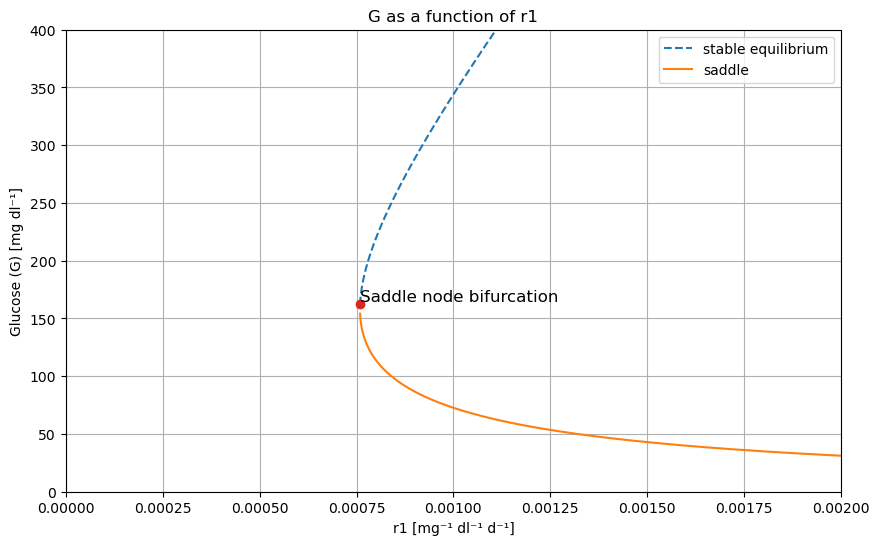
\includegraphics[width=0.7\textwidth]{Img/betadynamic.png}
    \bicaption{胰$\beta$细胞动力系统模型分岔。}{Pancreatic \(\beta\) cell dynamic system model bifurcation.}
    \label{fig:bifurcation}
\end{figure}

由于胰$\beta$细胞数量变化较慢(一般以天为单位观测),在连续血糖监测的过程中,我们以每次进食为数据分段标准,因此我们可以考虑将$\beta$细胞视为常量,仅考虑葡萄糖-胰岛素动力系统\cite{huard2022mathematical}。我们可以得到如下动力系统模型:
\begin{equation}\label{11}
    \begin{aligned}
        \dot{G} & = a_0-a_1G-a_2GI+\frac{a_3}{a_4+I^p},  \\
        \dot{I} & = \frac{b_1 G^2}{G^2 + b_2^2} - b_3 I,
    \end{aligned}
\end{equation}

对于因为对胰岛素敏感性降低而引起的糖尿病,如图\ref{fig:hyperglycemia}所示,最终血糖的稳定浓度和胰岛素的稳定浓度都高于正常人。
\begin{figure}[H]
    \centering
    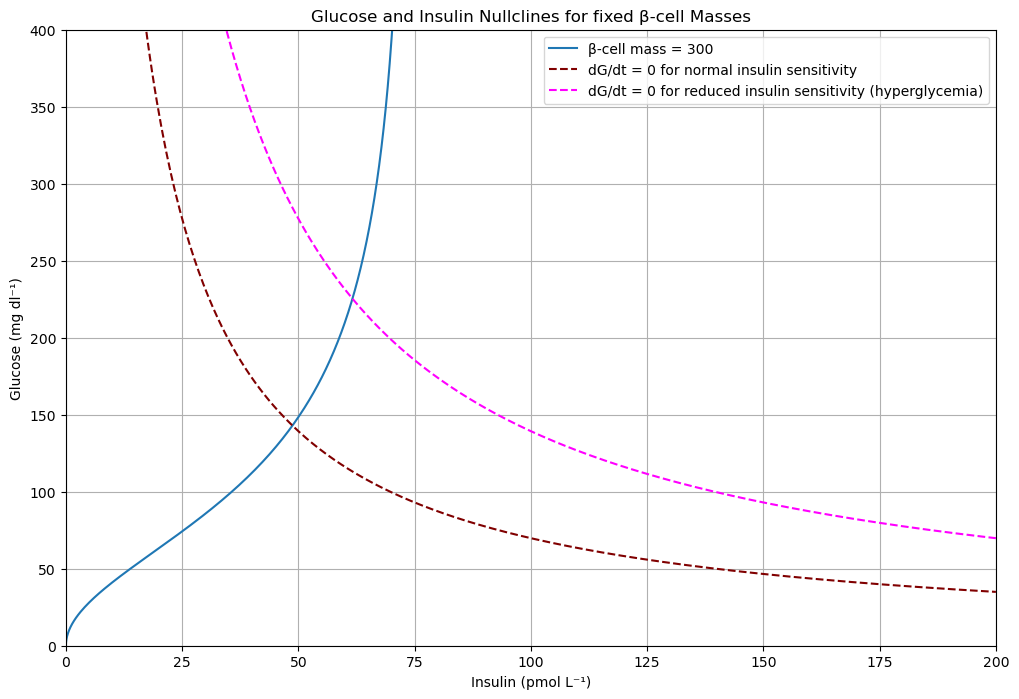
\includegraphics[width=0.7\textwidth]{Img/hyperglycemia.png}
    \bicaption{胰岛素敏感性降低引起的糖尿病。}{Diabetes caused by decreased insulin sensitivity.}
    \label{fig:hyperglycemia}
\end{figure}

对于常见的二型糖尿病,可能是胰$\beta$细胞数量较少,如图\ref{fig:beta}所示,也可能是胰岛素分泌速率更低,如图\ref{fig:lessinsulin}所示,最终血糖的稳定浓度高于正常人,胰岛素浓度低于正常人,可以通过外界注入胰岛素来使血糖值正常。
\begin{figure}[H]
    \centering
    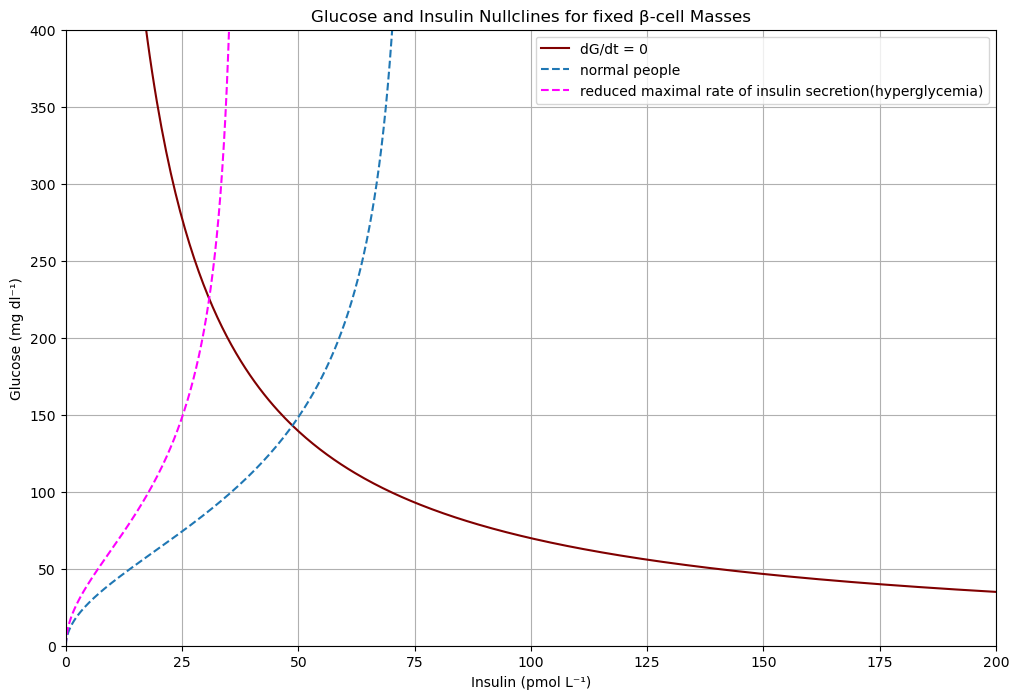
\includegraphics[width=0.7\textwidth]{Img/lessinsulin.png}
    \bicaption{胰岛素分泌速率降低引起的糖尿病。}{Diabetes caused by decreased insulin secretion rate.}
    \label{fig:lessinsulin}
\end{figure}
\section{模型参数估计方法}
在实际应用中,我们需要根据实验数据估计模型参数。在估计模型参数时,我们通常使用最小二乘法来拟合模型。

\begin{defn}[最小二乘法]
    给定一组实验数据$(x_i, y_i)$,我们的目标是找到一组参数$\theta$,使得模型预测值$f(x_i, \theta)$与实际观测值$y_i$之间的残差平方和最小。最小二乘法的目标函数为:
    \begin{equation}
        \theta^* = \arg\min_{\theta} \sum_{i=1}^{n} (y_i - f(x_i, \theta))^2,
    \end{equation}
\end{defn}

在编程中,我们通常使用数值优化算法来求解最小二乘问题。常用的数值优化算法包括梯度下降法、共轭梯度法、牛顿法等。这些算法可以有效地求解高维非线性最小二乘问题,帮助我们估计模型参数。

我们先将动力系统模型(\ref{11})转化为差分方程形式,然后根据实验数据使用最小二乘法估计模型参数。具体步骤如下:

\begin{enumerate}
    \item 将动力系统模型(\ref{11})转化为差分方程形式:
          \begin{equation}
              \begin{aligned}
                  G_{t+1} & = G_{t-1} + 2\Delta t \left(a_0-a_1G_t-a_2G_tI_t+\frac{a_3}{a_4+I_t^p}\right), \\
                  I_{t+1} & = I_{t-1} + 2\Delta t \left(\frac{b_1 G_t^2}{G_t^2 + b_2^2} - b_3 I_t\right),
              \end{aligned}
          \end{equation}
    \item 给定一个人一段时间没有外界糖类输入的血糖值向量$(G_i,t_i)_{i=1}^n$,通过差分方程算出来的葡萄糖数值为$f(\theta)$,是一个向量,长度为$n$,对应的是$t_i$时间通过差分方程算出来的血糖值,定义损失函数:
          \begin{equation}
              L(\theta) = \Vert\mathbf{G}-f(\theta) \Vert_2^2+\epsilon\Vert \theta \Vert_2,
          \end{equation}
          其中$\epsilon$是正则化参数,用于防止过拟合。
    \item 我们可以使用梯度下降法求解。
          \begin{equation}
              \theta^* = \arg\min_{\theta} L(\theta),
          \end{equation}
\end{enumerate}

在实际编程中,我们可以使用pytorch(2.3.0版本)中的$DFNet$类来辅助进行参数估计:
 \begin{algorithm}[H]
        \caption{模型参数估计}
        \begin{algorithmic}[1]
            \State 初始化模型: $model \leftarrow DFNet()$
            \State 加载模型状态: $model.\text{load\_state\_dict}(\text{torch.load}('model.pth'))$
            \State 初始化优化器: $optimizer \leftarrow \text{torch.optim.SGD}(model.parameters(), \text{lr}=2e-12, \text{weight\_decay}=0.01)$
            \State 加载数据: $data$
            
            \State 初始化最佳损失: $best$
            \State 初始化最佳参数: $best\_params \leftarrow$ (model.a0, model.a1, model.a2, model.b1, model.b2, model.b3, model.I0)
            
            \For{$i = 0$ 到 $49$}
                \State 计算损失: $loss \leftarrow model.loss(data)$
                \State 清零梯度: $optimizer.\text{zero\_grad}()$
                \State 反向传播损失: $loss.\text{backward}()$
                \State 更新模型参数: $optimizer.\text{step}()$
                \If{$loss < best\_loss$}
                    \State 更新最佳损失: $best\_loss \leftarrow loss$
                    \State 更新最佳参数: $best\_params \leftarrow$ (model.a0, model.a1, model.a2, model.b1, model.b2, model.b3, model.I0)
                \EndIf
                \State 打印迭代次数和损失: $\text{print}(\text{f'迭代 } \ i \ \text{次,损失: } \ loss.item())$
            \EndFor
        \end{algorithmic}
    \end{algorithm}
 
    其中我们使用$torch.optim.SGD$来定义优化器,其中SGD表示随机梯度下降。

随机梯度下降(Stochastic Gradient Descent, SGD)是一种用于优化机器学习和深度学习模型的算法,通过以下步骤迭代更新模型参数:
\begin{enumerate}
    \item 初始化模型参数 $\theta$。
    \item 在每次迭代中,随机抽取一个训练样本 $(x_i, y_i)$,计算对应的梯度 $\nabla L(\theta; x_i, y_i)$,并根据梯度更新模型参数。
\end{enumerate}

参数更新公式为:
\begin{equation}
    \theta_{t+1} = \theta_t - \eta \nabla L(\theta_t; x_i, y_i),
\end{equation}
其中:
\begin{itemize}
    \item $\theta_t$ 是第 $t$ 次迭代时的模型参数。
    \item $\eta$ 是学习率。
    \item $L(\theta; x_i, y_i)$ 是第 $i$ 个样本的损失函数。
    \item $\nabla L(\theta_t; x_i, y_i)$ 是损失函数对参数 $\theta$ 的梯度。
\end{itemize}

该算法的优点具体表现为:

\begin{itemize}
    \item 计算效率高:每次更新只需计算一个或少量样本的梯度,适合大数据集。
    \item 内存需求低:每次只需存储一个或少量样本的数据,节省内存。
    \item 能避免局部最小值:由于引入了随机性,能够帮助跳出局部最小值,找到全局最优解。
\end{itemize}

该算法的缺点包括:

\begin{itemize}
    \item 噪声较大:每次仅使用一个或少量样本,梯度估计有较大噪声,收敛过程不如批量梯度下降稳定。
    \item 超参数调节复杂:学习率等超参数对模型性能影响较大,需要仔细调节。
\end{itemize}

    我们使用$zero\_grad$方法清零梯度,以避免梯度累积。然后我们使用反向传播函数($backward$)方法计算梯度,其使用pytorch内置的求梯度方法\cite{paszke2017automatic},并使用SGD中内置的$step$函数更新模型参数。在训练过程中,我们保存最佳损失和最佳参数,并在训练结束后打印最佳参数。最后,我们保存模型状态,以便在以后的预测中使用。
